\poemtitle{EP 2: Ru D. and June's Delivery Service - How Wool met June and Ru D.}

Before the event I am about to describe, nobody even knew about the existence of mechanic Wool.
This is simply because during his childhood, he once visited a factory, where he became fascinated by a vintage car. 
That car was so extraordinary to him, that he discreetly drove away with it (he was already very smart as a kid), and nobody could ever find him, or the car. 


At that time, people suspected it was the dangerous but powerful engineer Dr. Melon Dusk who had stolen the car, possibly kidnapping the curious kid on the way. Too afraid to investigate further, people gave up on finding the child.


Far from feeling lonely, he soon chose a new name, Wool Lionson, and built an army of friends, all with their own personality: energetic danger detector Sunny, easygoing fire extinguisher Windy, quiet lock-unlocking tool Ninja, and many others.
You may wonder, why don't we just leave him alone with his new life?
Well, his life was just about to change. 

\begin{center}
    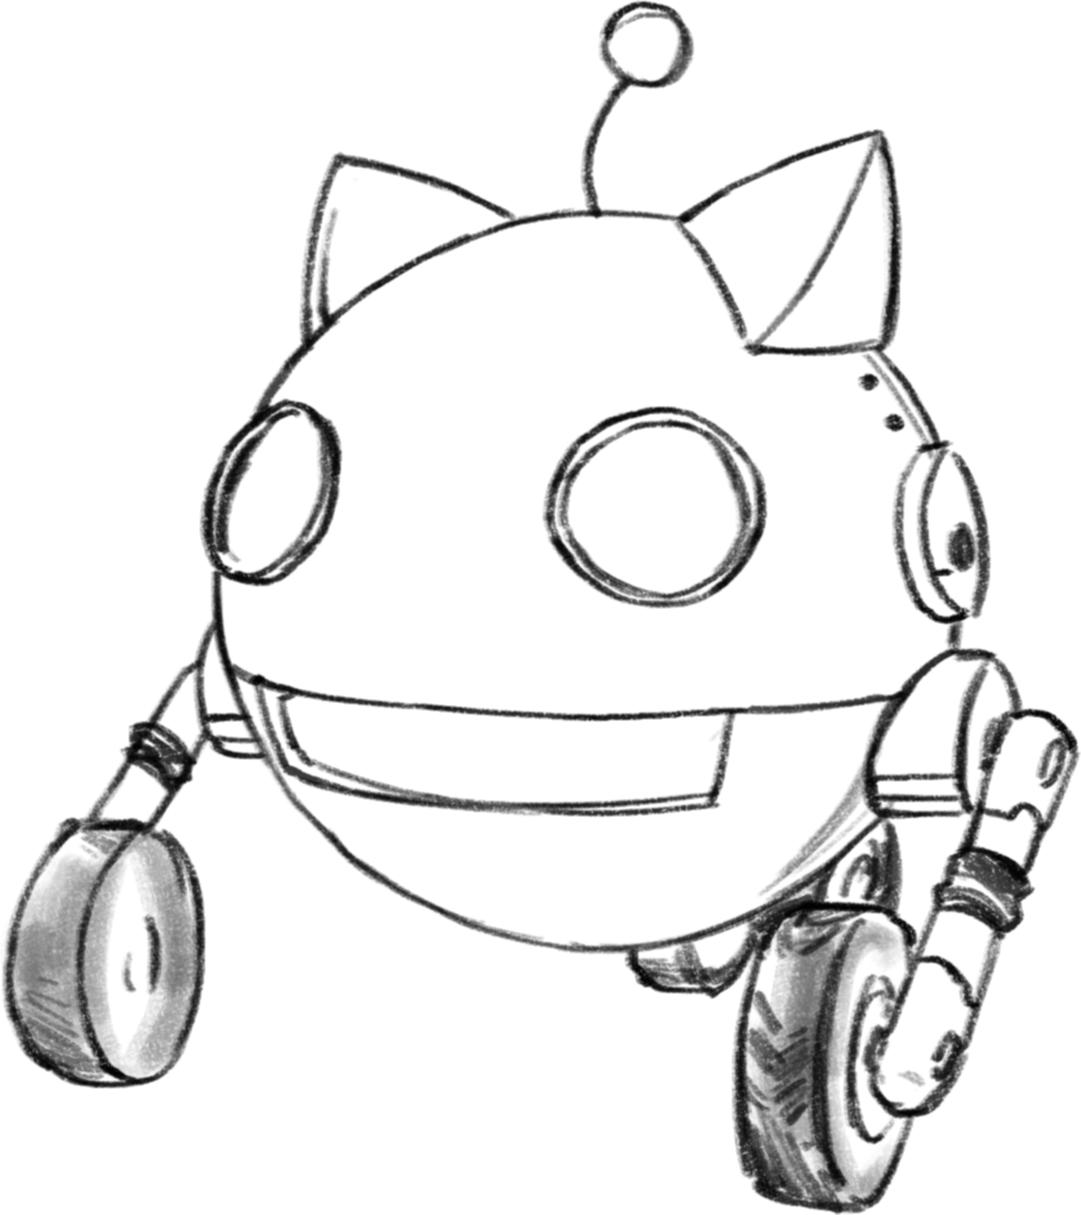
\includegraphics[height=.2\textheight]{Assets/wfbw_kirby}    
\end{center}

Wool had ordered a package with essential raw materials.
Usually, the delivery agents knew that they simply needed to deposit the packages in his interactive mailbox Kirby, without greeting Wool or anything. Kirby could finish the remaining paperwork and sign the packages, so delivery agents loved that little mailbox. In some circumstances, Kirby was even able to impersonate other people's signatures, but that's another story.


This time though, it was agent Ru D. who had been assigned to deliver the package. 
Ru D., who had just met scientist June, decided to show her his typical workday, as June had recently lost her job.
However, June had quit her job in such a dramatic way, that Ru D. and her were being hunted by government agents.
As they arrived at Wool's place, Ru D. felt surprised by the poor state of the location: 

``What a dumpster. How would anyone want to live here?'' he wondered. 

But June seemed charmed: ``I think this city is lovely, with so many pigeons! There's even a CK Wing's! Can we stop there? I'll get 12 cheese nuggets and this week's Happy Wing toy! What are you ordering?'' she asked.

But Ru D. was not hungry. Preoccupied by his task, he decided the quickest way to deliver his package would be the old-fashioned way. 
Ru D. knocked at the door, but no one answered. To help, June used her sonic weapon to play her latest song, so it would be audible by anyone in the city.
Sunny's alarm went along great with June's song, it was just as if they sang a duet together.

\begin{center}
    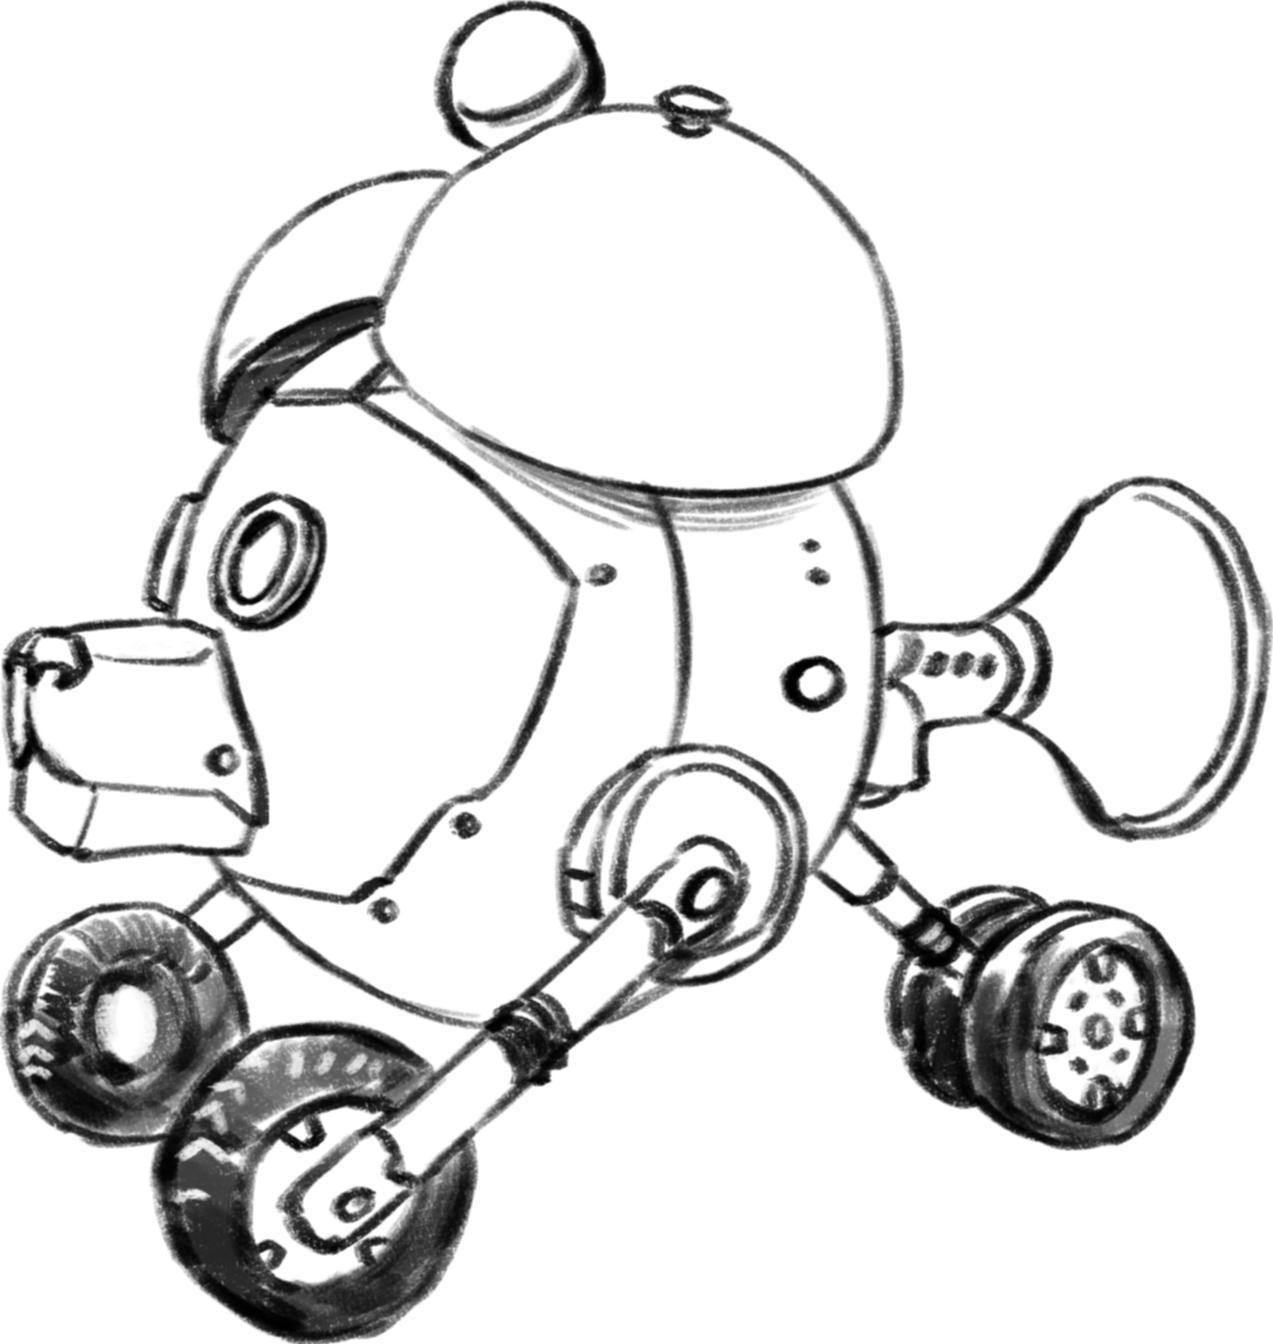
\includegraphics[height=.2\textheight]{Assets/wfbw_sunny}    
\end{center}


``Are you crazy???'' Ru D. shouted and gesticulated, so June stopped her engine. ``The government agents are going to find us for sure!'' he added.\\
``But... You just talked for hours and hours about how a job well-done is more satisfying than anything blah blah blah... And bragging about being the best newcomer employee of the year, so boring!'' June replied.


Wool approached them, looking furious.

``HOW DARE YOU SCARE MY LITTLE SUNNY??? AND INTERRUPT MY WORK???'' he yelled.\\
``Yeah yeah, sorry about that. Could you sign this package? We're kind of in a hurry.'' Ru D said, as the government ships were dangerously approaching.\\
``Oh no, not those government guys again!'' Wool complained. ``They keep bothering me about unpaid import fees on my packages. And everytime the fees increase!''\\
``Don't worry,'' June ensured. ``We're taking care of that. It's part of our job after all, just make sure to leave us positive feedback ok?''\\
``Wait... What?'' Ru D. asked, looking very worried.


Too late, as June had already assembled a cannonball from her tools, and began shooting at the ships.\\
``Fascinating,'' Wool observed, ``how on Earth could you build such a powerful engine from this tiny amount of materials? You're not precise enough though, let me show you how to adjust your weapon to the proper angle, for optimal impact.''\\
``These two are so weird, of course they're getting along'', Ru D. remarked. ``Alright, I guess there's no choice, I need to find a way to buy time so we can get out of here,'' he concluded.


Unfortunately, there were many agents, it was impossible to fight all of them. Furthermore, Ru D.'s ship had been greatly impacted by the government missiles.
As the agents started dropping fire bombs, Wool shouted to his fire extinguisher ``Windy, blow these things away from my house!''. \\ 
Windy then skillfully redirected the bombs towards CK Wing's, thus preserving Wool's house and our protagonists.

\begin{center}
    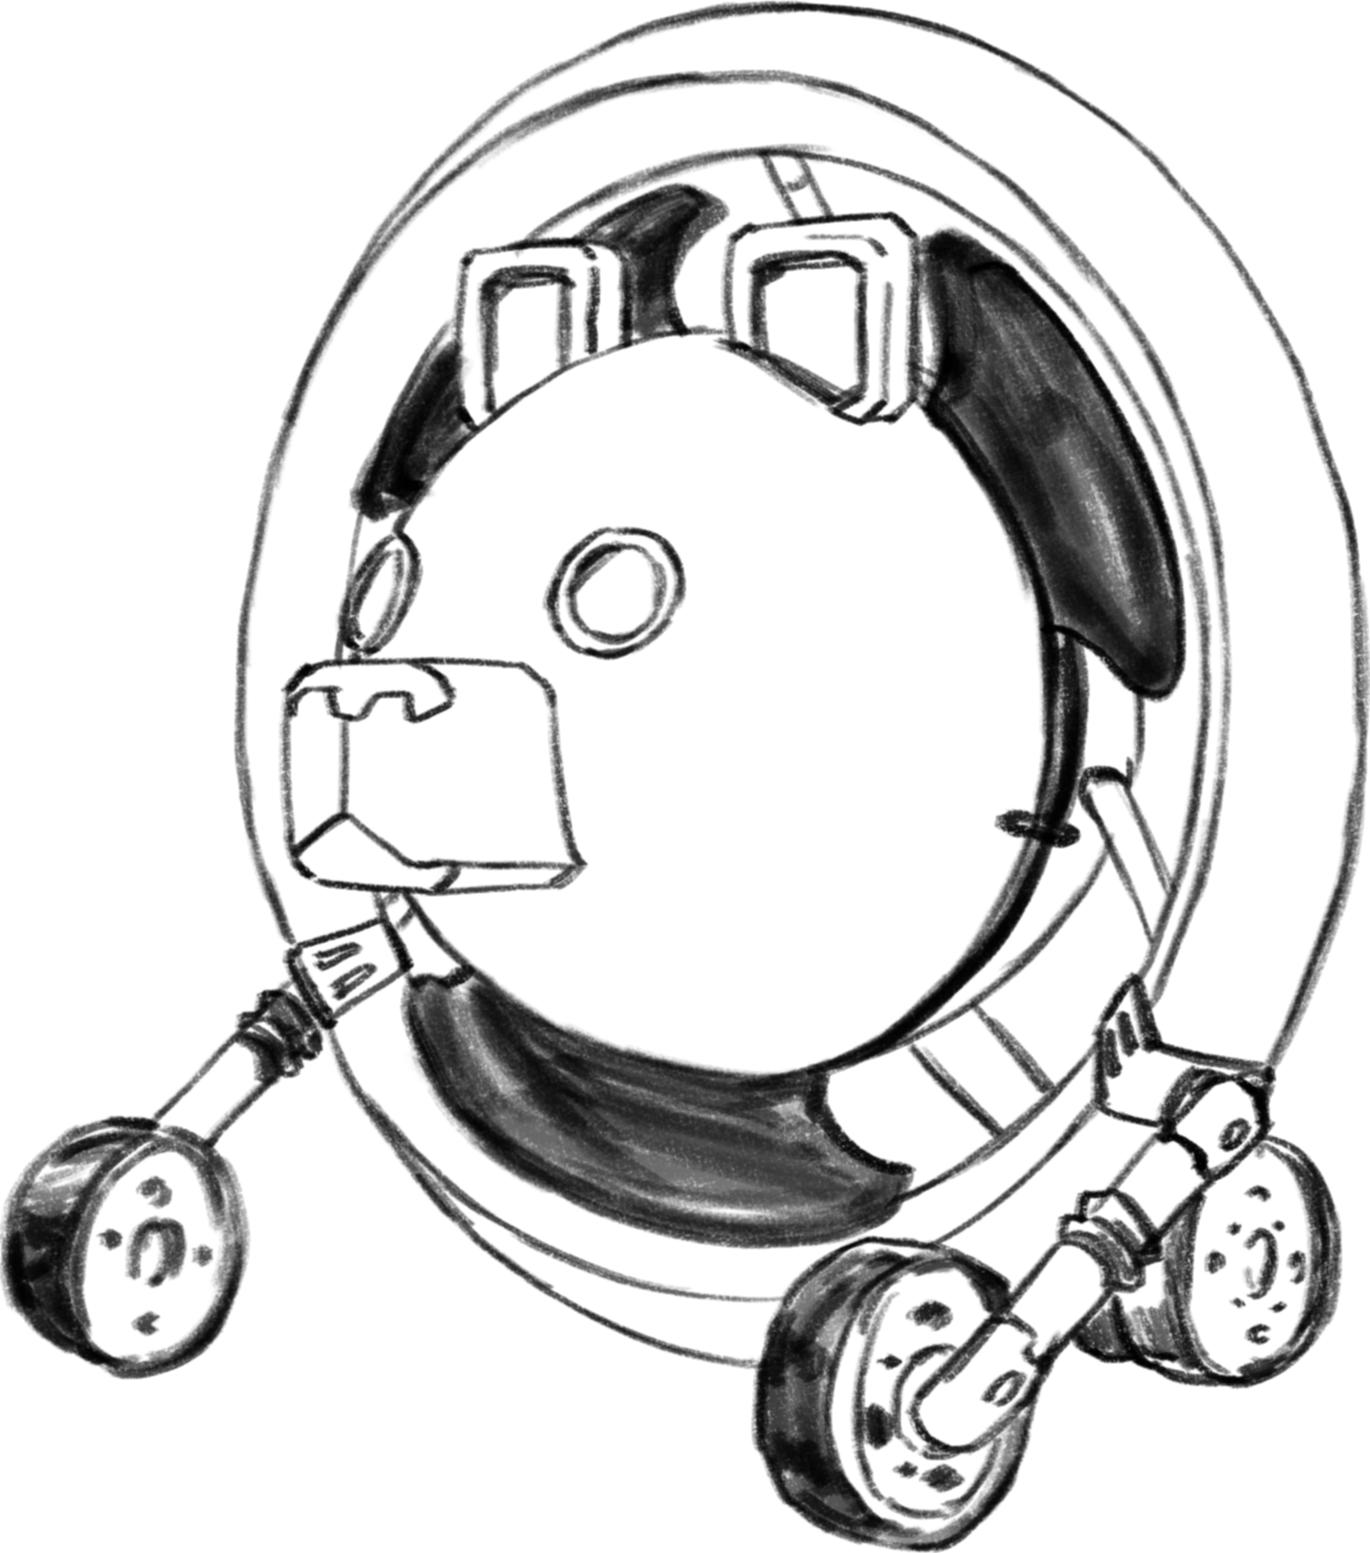
\includegraphics[height=.2\textheight]{Assets/wfbw_windy}    
\end{center}


``Guys, we must escape NOW!'' Ru D. screamed. ``There are more of them coming! Thankfully that was my last delivery task for this round!''\\
They all ran inside Wool's house, and Ninja moved by itself, to open a door on the floor.\\
``This is my secret blast shelter. They won't find us here, the soundproofing is quite good,'' Wool said.\\
They jumped inside, then Ninja locked the door.\\
``Is there another exit from here?'' Ru D. asked.\\
``Yes, to my secret kitchen,'' Wool replied.\\
``How many secret...'' June started.\\
``We don't have time for this.'' Ru D. interrupted ``Is there a way to escape the city from the secret kitchen?'' he asked.\\
``The secret kitchen has another exit to my living room.'' Wool replied.\\
``Oh so you mean we can go to the secret kitchen, making sure to lock all the doors when we don't need them anymore...'' June began.\\
``Yes that's it! The moving key in your hand, can you control it so that it can move by itself from one room to another?'' Ru D. asked.\\
``You're talking about Ninja right? True, my agile friend will be able to help us,'' Wool replied.\\
``So as June says, first we move to the secret kitchen, making sure all the unused doors are locked...'' Ru D started.\\\\
\clearpage  % depends on page format
``Then SURPRISE!!!! We go to the living room, and shoot all the agents! They will never expect us to appear from the secret kitchen hahahahahahaha,'' June interrupted.\\
``How can your initial observation be so accurate, but your conclusion so wrong?'' Wool asked. ``Indeed, while we are in the secret kitchen, Ninja can open the door to the blast shelter and make some noise, so that they all think we are hiding there. We will wait until they are all in the shelter, then Ninja can trap them inside. Also, the package in your hands is actually the key to our escape, as it contains the replacement for the navigation system of my ship! I just need to plug it in... as long as I connect the cables correctly, it is good to fly,'' Wool explained.\\
``Hey, are you sure this is safe? What happens if we mess up the connections?'', Ru D. worried.\\
``Don't worry,'' June ensured. ``He's taking care of that. It's part of his job after all, just make sure to write a will and...'' she added, but as Ru D. began to panic, Wool interrupted her:\\
``Luckily, there is a simulation mode. Thanks to that we can find the mistakes in advance so we are safe. The system will say in a cute voice `Let's try again!'.''\\
``Awesome! You quickly decide on what to keep with you, then reach your ship and take care of June. I'll join you guys after throwing some sticky traps to slow down unexpected visitors, so we all have time to escape,''  Ru D. replied.\\
Wool's eyes were shining from the soundness of Ru D.'s reasoning. \\
``Wow, these two are meant to become the best of friends,'' June thought.

\begin{center}
    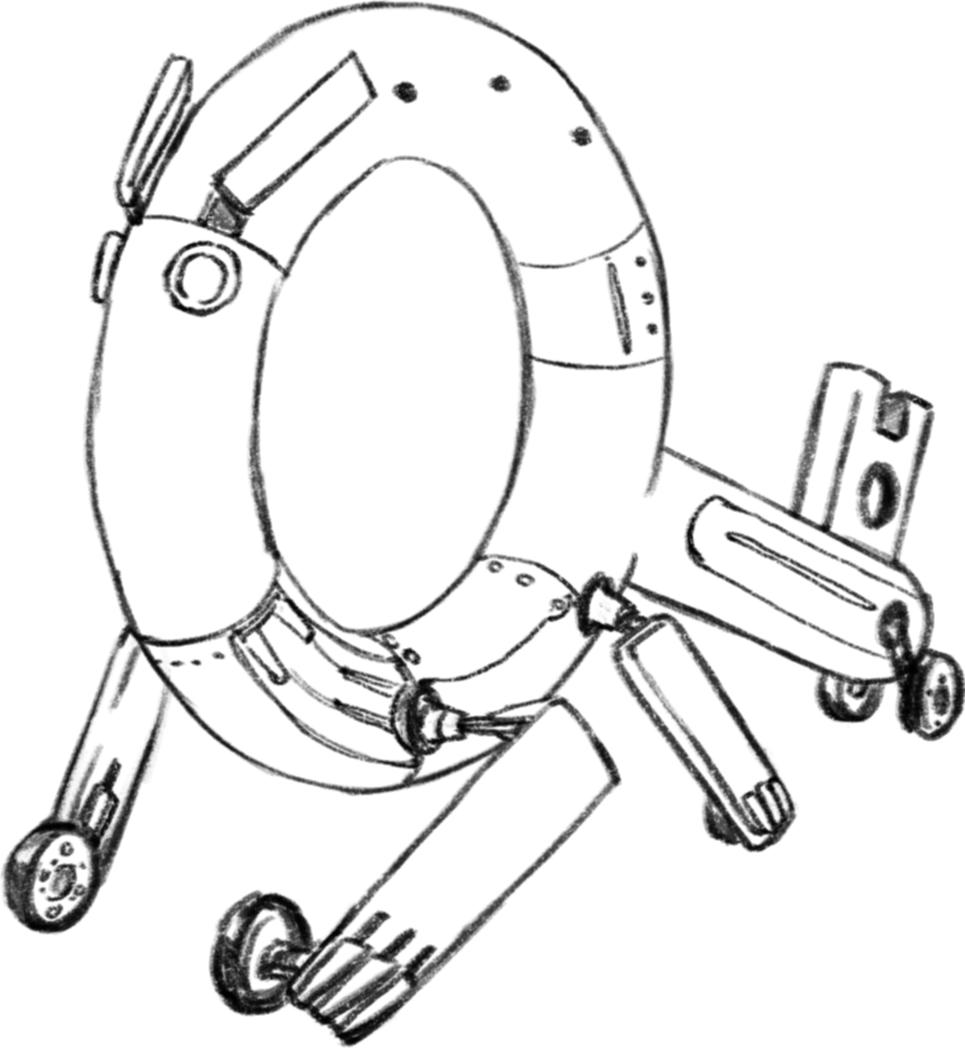
\includegraphics[height=.2\textheight]{Assets/wfbw_ninja}    
\end{center}

\clearpage  % depends on page format
As they were carefully preparing their exit in the secret kitchen, June asked:\\
``Have you already worked with a Squirelly suit? No need for all these secret rooms when you can use this suit to jump, climb and hide practically anywhere! Also feed yourself nutritious meals with the nut dispenser! And make powerful attacks without being seen! But being unnoticed is not very fun, so I never use the Squirelly for myself.''\\
``Don’t you need Cosmonol Glue to make it?'' replied Wool. ``This component is very hard to find and considered dangerous goods, forbidden for shipping. I would need to travel for a while to find it.''\\
``Well today is the perfect day for some fresh air! Come with us! I can show you where to find all the components! I can show you the world! Shining shimmering and super rare gears!'', said June with stars in her eyes.\\
``For real? I also wanted to try uranium cyanade to fuel my machines. The most economical, powerful power source, but supposedly ‘hazardous’ so they won’t sell it here,'' a frustrated Wool replied.\\
``Well my house may not be the most pleasant place at the moment. Maybe I can travel with you for a little while, and wait for quieter days to return home.'' he concluded.

Back to executing the escape, their plan almost failed when June jumped to Wool's custom High-Res music player, trying to play one of her songs. But thankfully, Ru D. and Wool joined their forces to ensure the three of them could get out of the house.


As they crammed themselves into the ship, Wool began plugging all inputs and outputs of the navigation system without hesitation, as if he had done it many times in the past.
Right after Wool deactivated the simulation mode, ready to fly, Ru D. struggled to restrain June, who was trying to arrange the cables into a pigeon shape. This time, getting one cable wrong might have been fatal! 
\clearpage  % depends on page format
Once Wool was done, weird symbols appeared on the screen. ``We're ready'', he confidently asserted.\\
``Are you sure??? It doesn't seem right, why does the screen look like a ransom letter?'' Ru D. asked.\\
``You don't read pico-boustrophedon? It's a nice tool, unfortunately I don't have time to teach you right now, let's go!'' Wool replied.\\
As he pushed the lever, a slight hiss became louder, until the ship back started levitating slightly. Everyone looked a bit uncomfortable, until they heard a little `POP!', then the ship began to move swiftly through the air, as expected, of course.\\
``We'll start flying very close to the ground for a bit, to avoid detection. I know my way through the junkyard behind like nobody does, we'll be safe from pursuit,'' Wool affirmed.\\
The ship docked at Wool's container hidden nearby, and with their cargo they started moving through the junk canyons.

\begin{center}
    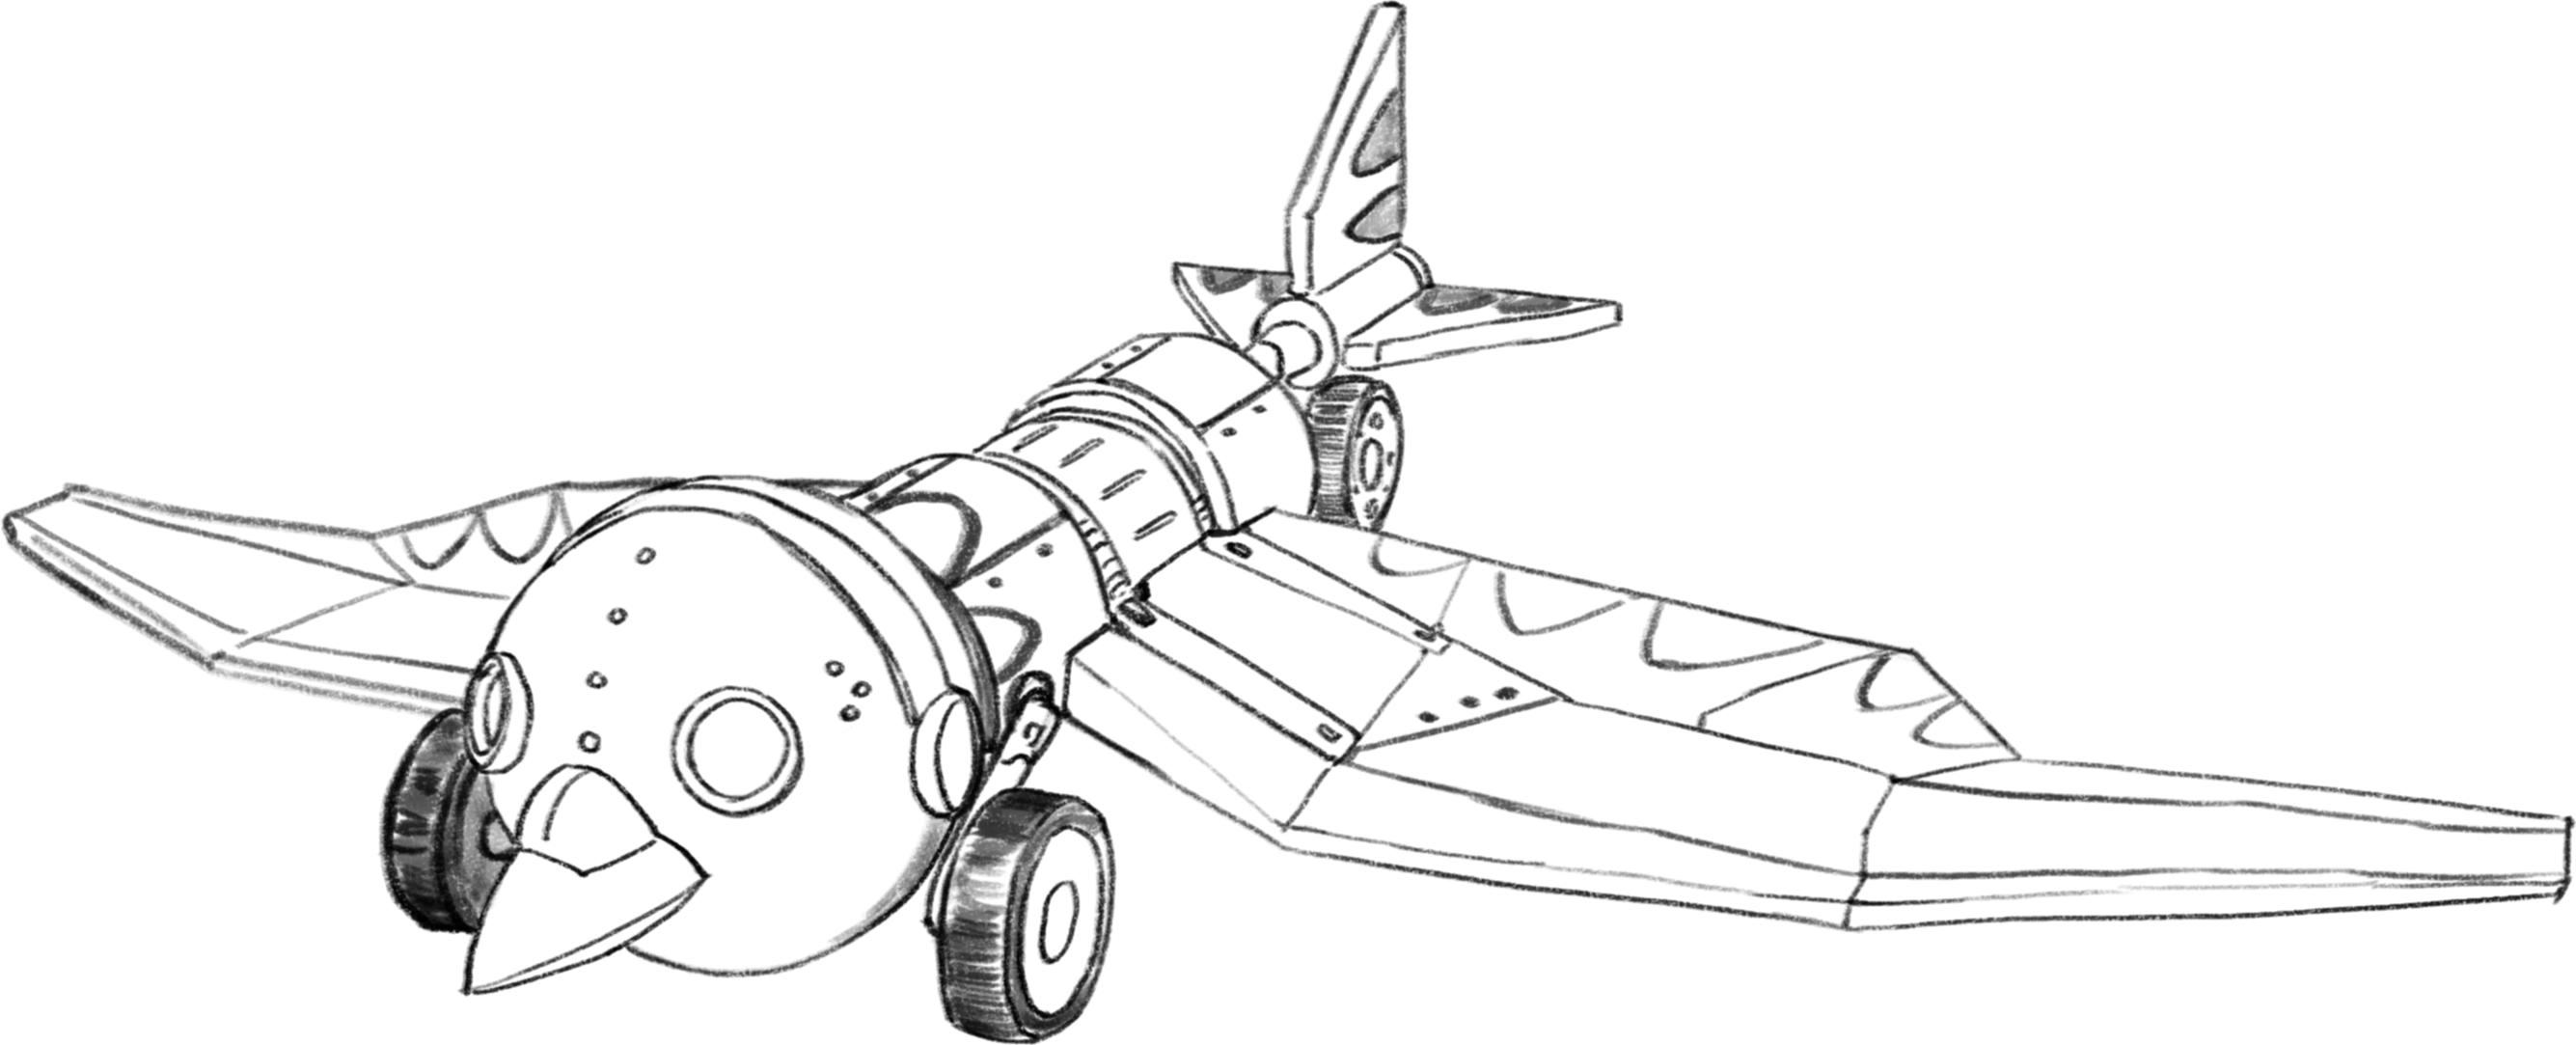
\includegraphics[height=.15\textheight]{Assets/wfbw_pigeon}
\end{center}
\begin{center}
    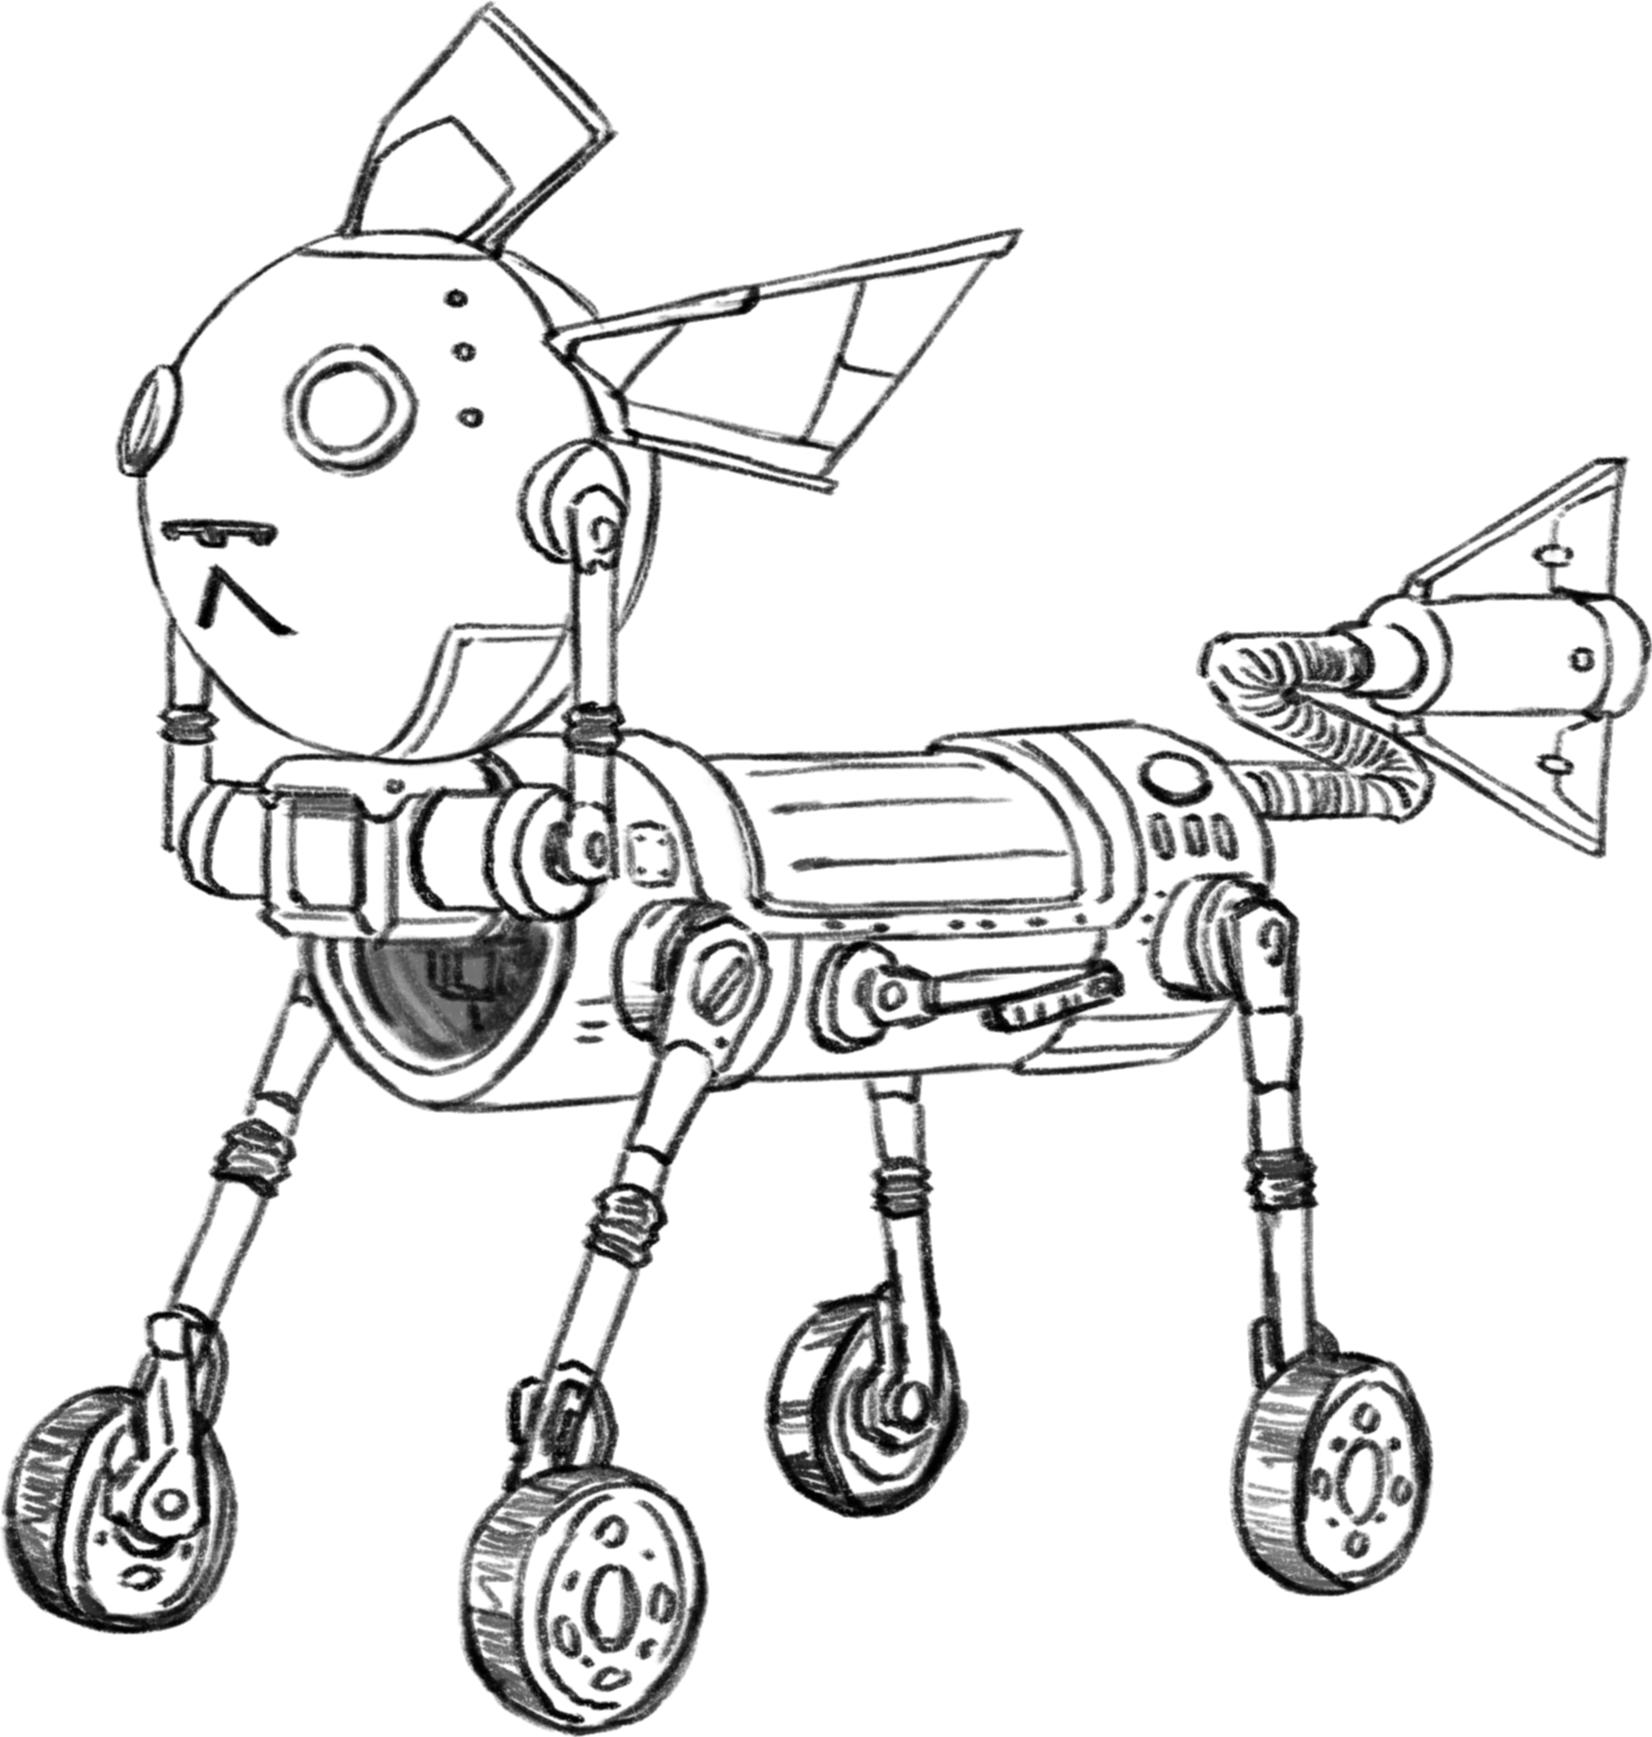
\includegraphics[height=.2\textheight]{Assets/wfbw_liqueon}
    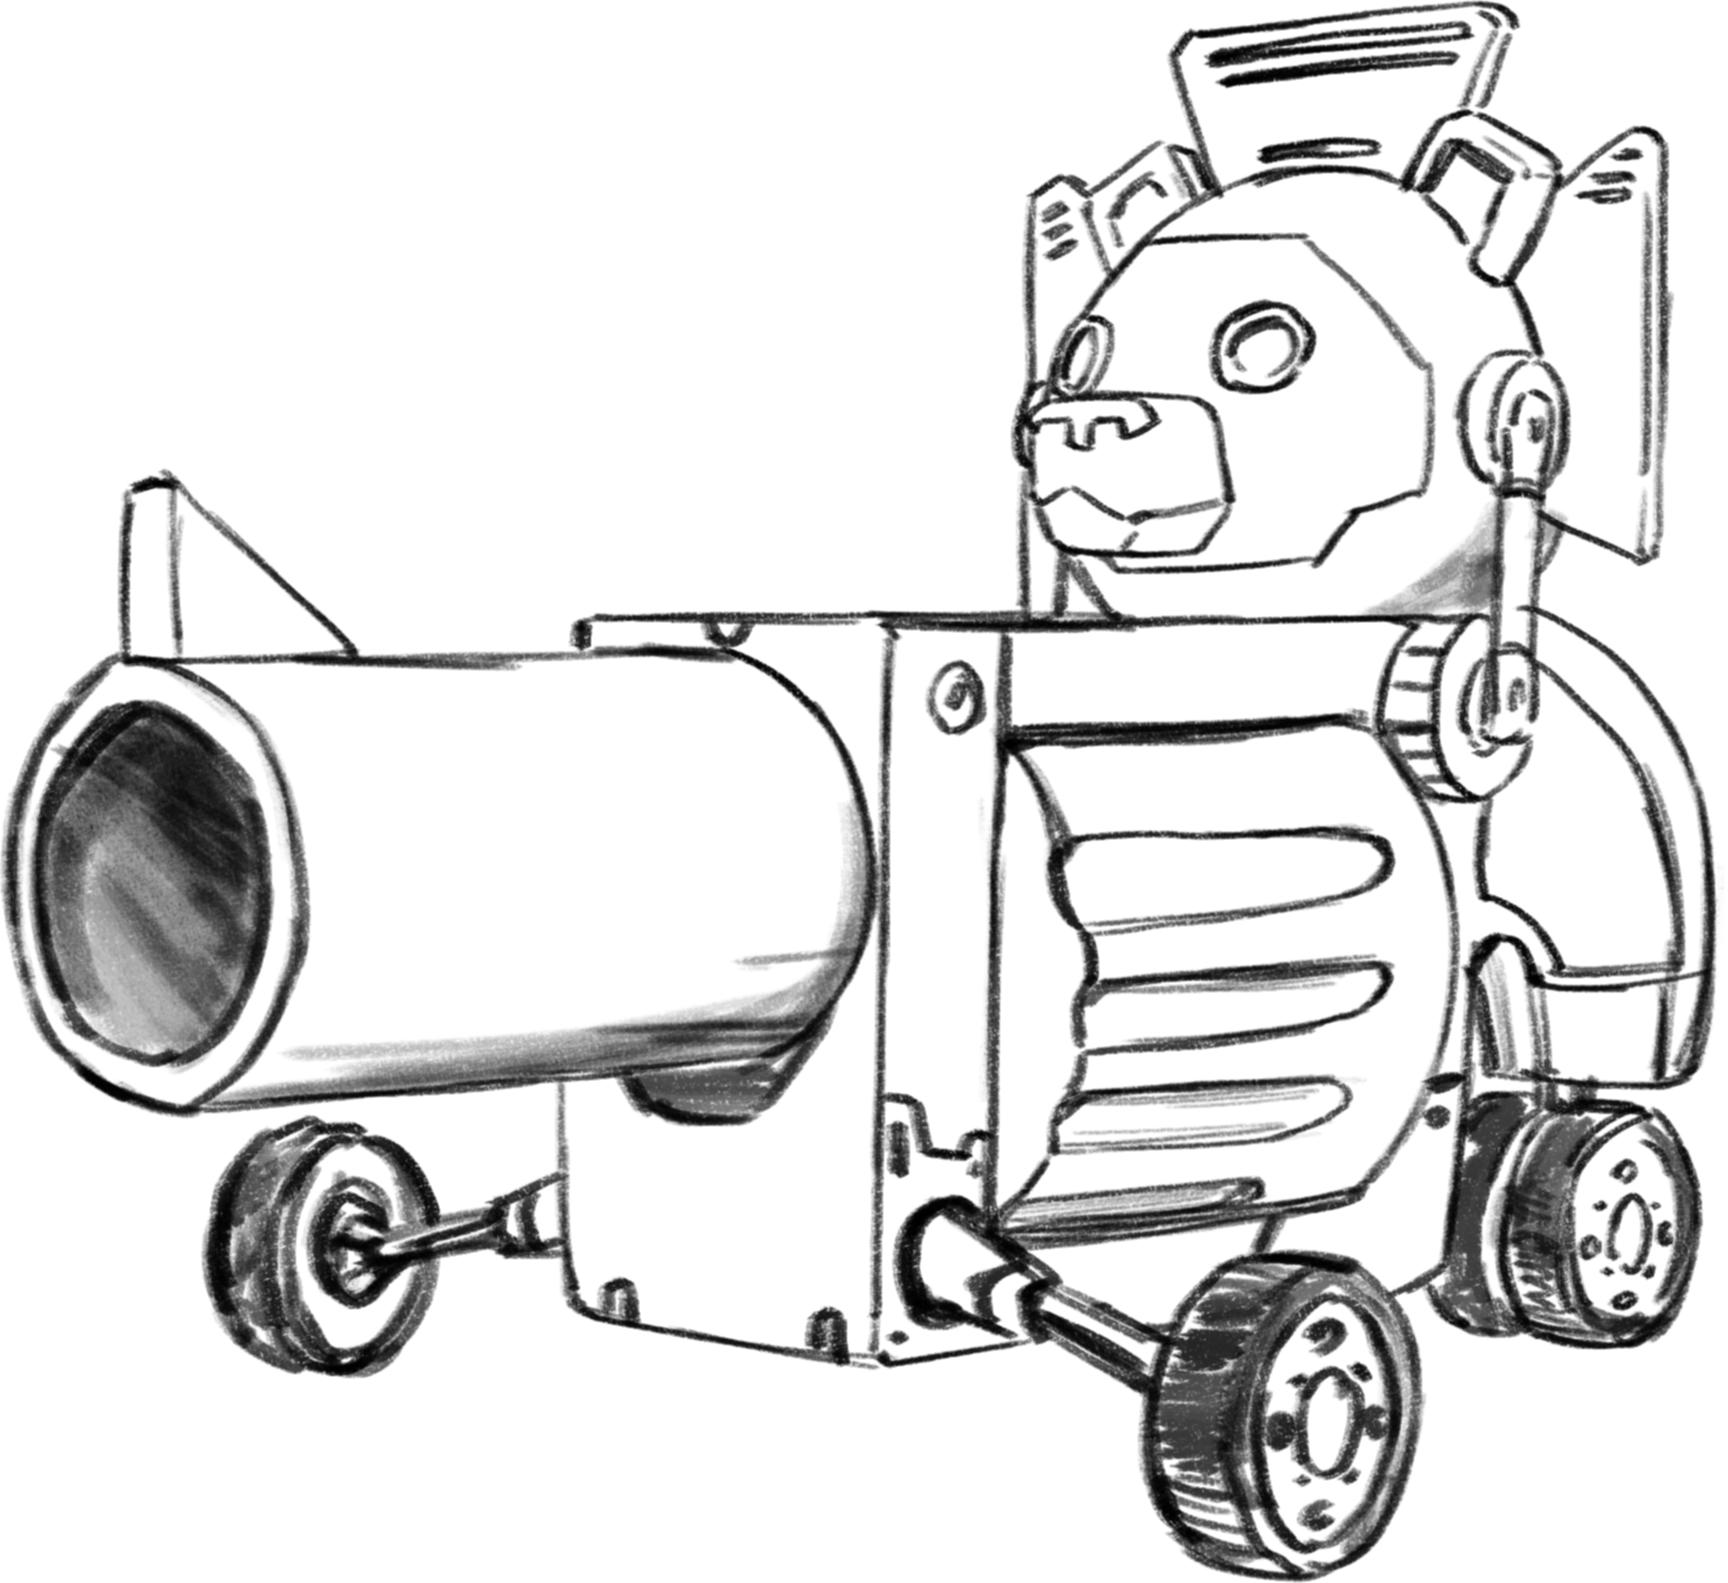
\includegraphics[height=.2\textheight]{Assets/wfbw_guneon}
\end{center}

As they reached the end of the junkyard, they slowly rose through the skies, and saw the city vanish into the distance.\\
Little green dots appeared on the ship's radar, and Ru D. started panicking, again:\\
``How can they be so fast??? Projectiles!!! Everywhere!!! So close! How can we go faster??? We’re dead meat!!!''\\
But Wool was smiling, and tearfully exclaimed:\\
``Liqueon! Guneon! Pidgeon! Windy! Ninja! Kirby! You all made it!!!! They’re not projectiles or enemies, they’re my friends!'' \\
``Oh okay… After lunatic nerds, now there are pets to take care of...'', Ru D. sighed.\\
``I see Sunny as well!!!! Ring the alarm Sunny, and sing with me! Tick tock, lalalalalala'', June began to sing (more like shout).


``How can these two curious humans get along so well? There simply isn't any logic to it'', Wool thought while looking at his city, looking smaller and smaller as they all flew away.

\begin{center}
    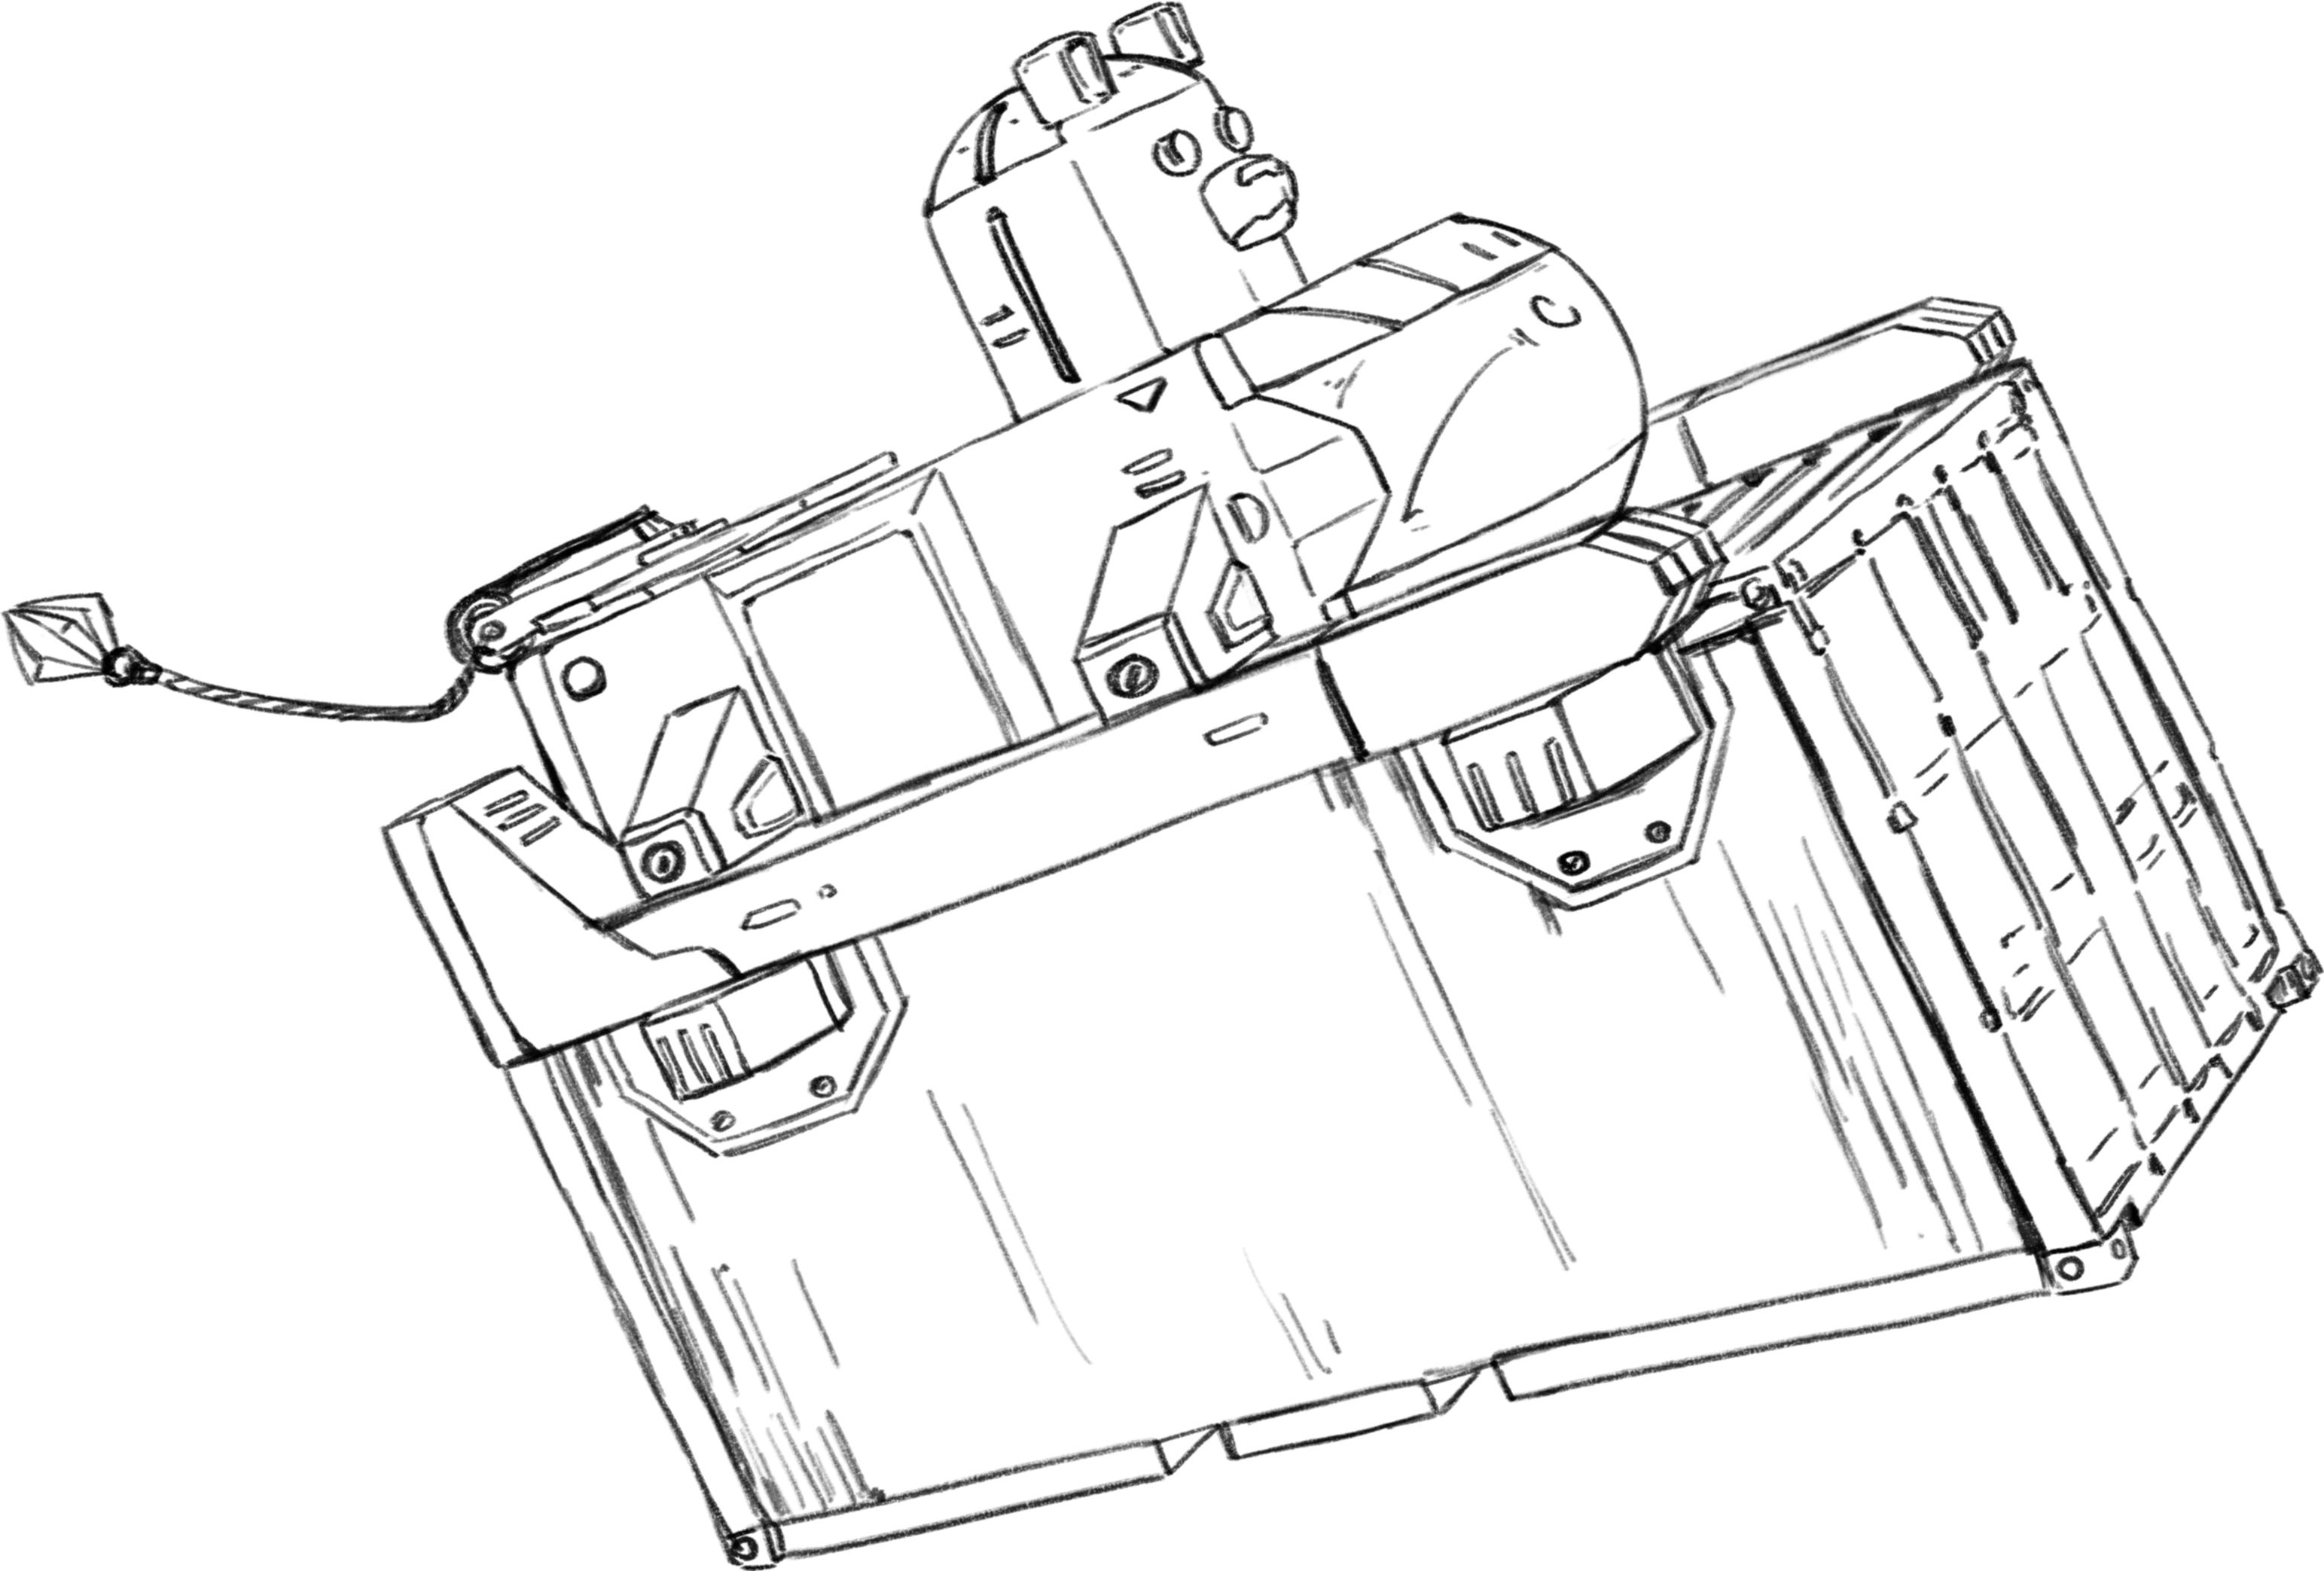
\includegraphics[width=.8\textwidth]{Assets/shipwithcontainer}    
\end{center}
